\documentclass[english,serif,mathserif]{beamer}
\usetheme[formal,deutsch]{s3it}

\usepackage[T1]{fontenc}
\usepackage[latin9]{inputenc}
\usepackage{babel}
\usepackage{graphicx}

\begin{document}

%% Optional Argument in [Brackets]: Short Title for Footline
\title[Short Title]{ Glance  }
\subtitle{Or: OpenStack's imaging service}

\author{ Tyanko Aleksiev \texttt{<tyanko.aleksiev@s3it.uzh.ch>}}

\date{\today}

\maketitle

\begin{frame}{Glance's role inside Openstack}

The OpenStack Glance service offers a REST API catalog enabling end users to:
\begin{itemize}
\item query,
\item register,
\item retrieve 
\end{itemize}
virtual machine images and their metadata. 

\end{frame}

\begin{frame}{Glance components: \textbf{glance-api}}

\textit{glance-api} is the main Glance service that exposes and makes available both:
 
\begin{itemize}
\item the metadata about registered images,
\item the image data itself. 
\end{itemize} 

\end{frame}

\begin{frame}{Glance components: \textbf{glance-registry}}

\textit{glance-registry} is an internal glance service. It is used 
by glance-api (v1.0) for image metadata:
 
\begin{itemize}
\item storing,
\item processing,
\item retrieval.
\end{itemize}

v2.0 of glance-api operates idependatly from glance-registry.

\end{frame}

\begin{frame}{Glance components: \textbf{Database}}

\textit{Database} is used for storing image metadata and is typically based on MySQL.

\end{frame}

\begin{frame}{Glance components: \textbf{Storage}}

\textit{Storage} is the repository for the real image files. 
Different storage types are supported:

\begin{itemize}
\item Local File System (which is the one used in this tutorial),
\item Ceph,
\item Swift,
\item Cinder,
\item HTTP,
\item Amazon S3,
\item others...
\end{itemize} 

\end{frame}

\begin{frame}{Glance: components interaction}

\centerline{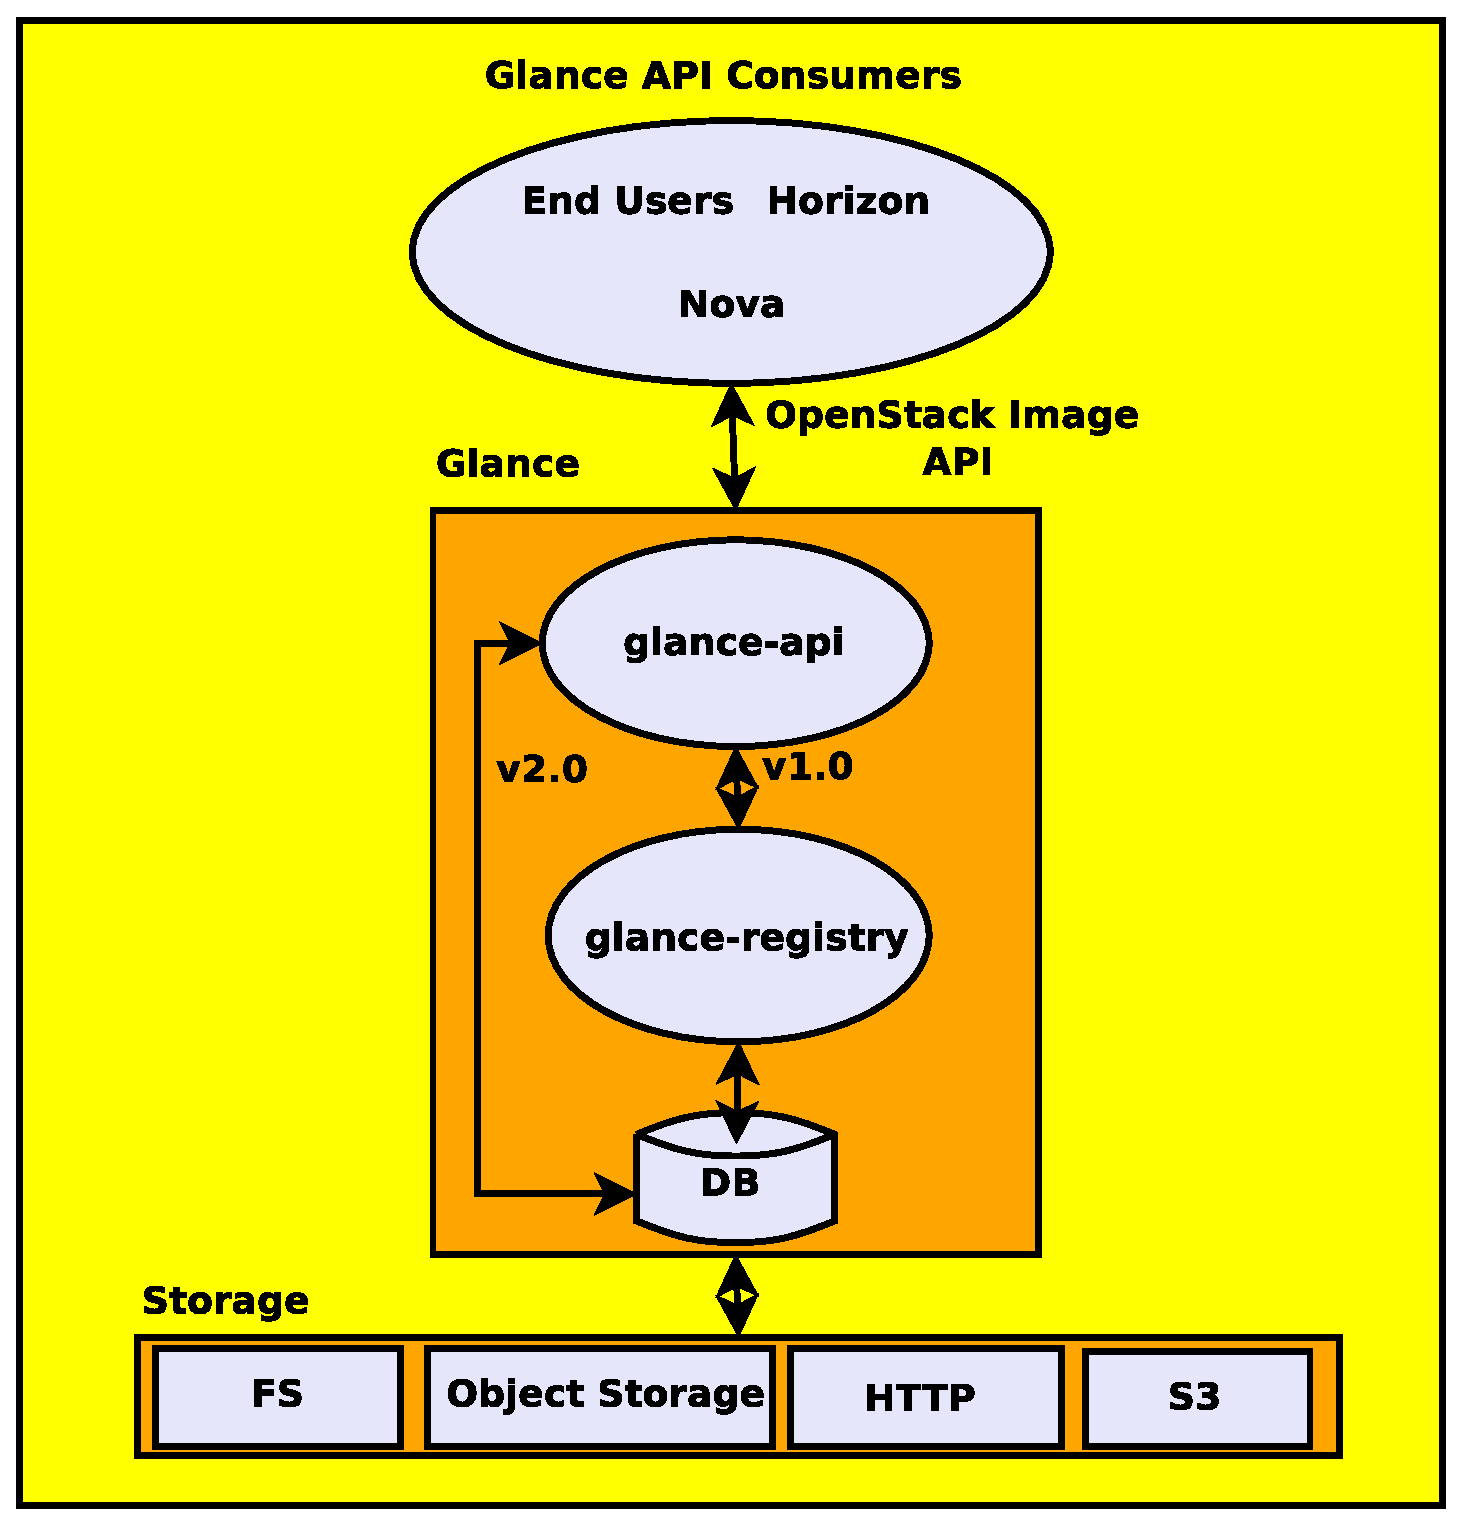
\includegraphics[scale=0.30]{glance.eps}}

\end{frame}

\begin{frame}{Notes and Remarks}

\begin{itemize}
\item Logs directory is: \texttt{/var/log/glance} 
\item Files you are going to edit often:
      \begin{itemize}
        \item glance-api conf. file is: \texttt{/etc/glance/glance-api.conf}
        \item glance-registry conf. file is: \texttt{/etc/glance/glance-registry.conf}
      \end{itemize}
\item We will see everything in more detail during the tutorial.
\end{itemize}

\end{frame}

\begin{frame}{Useful Links}

\begin{itemize}
\item {\color{blue}\href{http://docs.openstack.org/trunk/config-reference/content/ch\_configuring-openstack-image-service.html}{Configure Glance}}
\item {\color{blue}\href{http://docs.openstack.org/developer/glance/}{Glance Project Documentation}}
\end{itemize}

\end{frame}


\end{document}

%%% Local Variables:
%%% mode: latex
%%% TeX-master: t
%%% End:
